\chapter{Brain-Computer Interfaces (BCI)}

\section{Introduzione alle BCI}
Le interfacce Cervello-Computer stabiliscono un percorso di comunicazione diretta tra un cervello e un dispositivo esterno. Spesso dirette ad assistere, aumentare o riparare le funzioni cognitive o sensori-motorie umane.

\section{Tipologie di BCI}
Vi sono due grandi categorie per i sistemi BCI in base a come il cervello viene monitorato:
\begin{itemize}
    \item \textbf{Invasive}: Vengono impiantati elettrodi direttamente nel cervello. Hanno un'alta qualità di segnale (SNR molto alto) ma presentano rischi significativi per la salute del paziente e cicatrici nel tessuto cerebrale che nel tempo riducono l'efficacia del segnale.
    \item \textbf{Non-Invasive}: Utilizzano dispositivi posti all'esterno del cranio, come per l'elettroencefalografia (EEG). Pur avendo una risoluzione spaziale inferiore e maggiore suscettibilità al rumore (ad esempio rumori muscolari o movimenti agli occhi), offrono il grande vantaggio di essere sicure per l'utente, non richiedendo procedure chirurgiche.
\end{itemize}

\section{Componenti del Sistema BCI}
Un sistema tipico è composto da varie fasi di elaborazione:
\begin{enumerate}
    \item \textbf{Acquisizione del Segnale}: Tramite hardware dedicato e sensori (ad esempio, cuffie EEG).
    \item \textbf{Pre-processing ed Estrazione delle Features}: Rimozione del rumore (filtraggio, e.g. notch filter per rimuovere frequenza di rete) ed isolamento delle caratteristiche del segnale utili per decodificare l'intento.
    \item \textbf{Classificazione / Traslazione (Machine Learning)}: L'algoritmo traduce le feature estratte in un comando di controllo specifico usando modelli (come SVM o reti neurali).
    \item \textbf{Output del Dispositivo e Feedback}: Il comando viene eseguito (muovere un cursore, un braccio robotico, fare lo spelling di una parola) e all'utente viene dato un feedback visivo o tattile relativo alla sua azione, in modo tale che il suo cervello possa imparare ad adattare il segnale.
\end{enumerate}

\begin{figure}[h!]
    \centering
    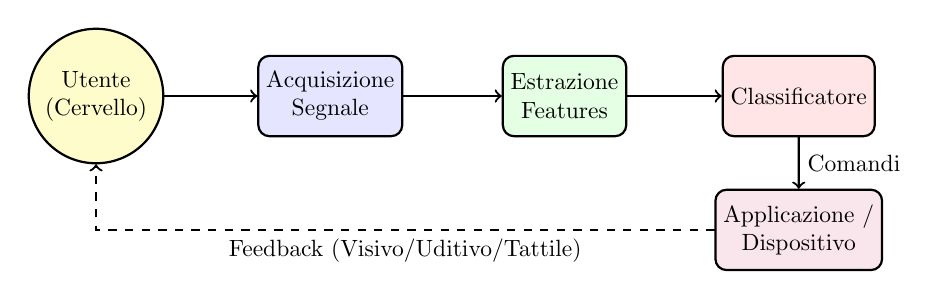
\begin{tikzpicture}[node distance=2.5cm, auto, thick, scale=0.85, every node/.style={scale=0.85}]
        \node[draw, circle, fill=yellow!20, minimum size=1.8cm, align=center] (user) {Utente \\ (Cervello)};
        \node[draw, rectangle, rounded corners, fill=blue!10, right of=user, node distance=3.5cm, minimum height=1.2cm, align=center] (acq) {Acquisizione \\ Segnale};
        \node[draw, rectangle, rounded corners, fill=green!10, right of=acq, node distance=3.5cm, minimum height=1.2cm, align=center] (proc) {Estrazione \\ Features};
        \node[draw, rectangle, rounded corners, fill=red!10, right of=proc, node distance=3.5cm, minimum height=1.2cm, align=center] (class) {Classificatore};
        \node[draw, rectangle, rounded corners, fill=purple!10, below of=class, node distance=2cm, minimum height=1.2cm, align=center] (app) {Applicazione / \\ Dispositivo};

        \draw[->] (user) -- (acq);
        \draw[->] (acq) -- (proc);
        \draw[->] (proc) -- (class);
        \draw[->] (class) -- (app) node[midway, right] {Comandi};
        \draw[->, dashed] (app) -| (user) node[near start, below] {Feedback (Visivo/Uditivo/Tattile)};
    \end{tikzpicture}
    \caption{Ciclo \textit{Closed-Loop} del sistema Brain-Computer Interface.}
\end{figure}

\section{Bande di Frequenza EEG}
Quando si analizzano segnali cerebrali non-invasivi, i tracciati EEG vengono usualmente divisi in bande di frequenza, ciascuna associata a determinati stati mentali:
\begin{itemize}
    \item \textbf{Delta ($\delta$) ($<4$ Hz):} Sonno profondo in adulti, o tracciati anomali da vegli (patologie).
    \item \textbf{Theta ($\theta$) ($4-7$ Hz):} Sonno leggero, sonnolenza marcata, attività prevalente in stadi di forte e profonda meditazione.
    \item \textbf{Alpha ($\alpha$) ($8-13$ Hz):} Stato di veglia ma rilassato, tipico di quando si chiudono gli occhi. È il ritmo più facile da individuare nei lobi occipitali.
    \item \textbf{Beta ($\beta$) ($14-30$ Hz):} Stato di veglia attiva, concentrazione, pensieri complessi o calcoli matematici.
    \item \textbf{Gamma ($\gamma$) ($>30$ Hz):} Percezione crociata, alto livello cognitivo o consolidamento di memorie rapide (meno usato a causa di artefatti muscolari coprenti alle stesse frequenze).
    \item \textbf{Ritmo Mu ($\mu$) ($8-12$ Hz):} Si sovrappone all'Alpha ma è localizzato sulla \textbf{corteccia motoria}. Si desincronizza (riduce di ampiezza) durante la preparazione o l'esecuzione di un movimento motorio (\textbf{Event-Related Desynchronization - ERD}).
\end{itemize}

\section{Sistema Internazionale 10-20}
Per standardizzare il posizionamento degli elettrodi sullo scalpo si usa il \textbf{Sistema 10-20}, basato su percentuali della distanza tra punti anatomici chiave (Nasion, Inion, e preauricolari). Le lettere indicano il lobo sottostante (\textbf{F} = Frontale, \textbf{C} = Centrale, \textbf{T} = Temporale, \textbf{P} = Parietale, \textbf{O} = Occipitale), mentre i numeri indicano l'emisfero:
\begin{itemize}
    \item \textbf{Numeri Dispari:} Emisfero Sinistro.
    \item \textbf{Numeri Pari:} Emisfero Destro.
    \item \textbf{Z (Zero):} Linea Mediana (Midline).
\end{itemize}

\section{Paradigmi BCI}
\subsection{Paradigma P300 Speller}
È uno dei sistemi BCI più famosi, permette a un utente di scrivere parole. Sfrutta il potenziale \textbf{P300}, una deflessione positiva dell'onda EEG (Event-Related Potential o \textbf{ERP}) che compare circa \textbf{300 ms} dopo uno stimolo atteso e raro (effetto \textbf{Oddball}).
\begin{itemize}
    \item \textbf{Funzionamento:} L'utente guarda uno schermo con una matrice $6 \times 6$ di lettere. Le righe e le colonne lampeggiano in modo casuale. Quando lampeggia la riga/colonna contenente la lettera desiderata, il cervello emette l'ERP P300. Intersecando riga e colonna la macchina deduce il carattere.
    \item \textbf{Averaging:} Poiché il P300 ha un'ampiezza di pochi $\mu V$, sommerso dal rumore di fondo (basso SNR), si richiede l'\textbf{Averaging} (media sincrona) su svariati flash. Mediando $N$ ripetizioni (trial), il SNR migliora di un fattore proporzionale a $\sqrt{N}$.
    \item \textbf{Attenzione:} Esiste l'attenzione \emph{Overt} (l'utente fissa direttamente la lettera spostando gli occhi) ed \emph{Covert} (l'utente tiene gli occhi fissi al centro, ma concentra l'attenzione mentale sulla lettera). Il sistema P300 con Overt attention è infinitamente più performante, dipendendo più da variazioni visive corticali.
\end{itemize}

\subsection{Paradigma Motor Imagery (Immaginazione Motoria)}
Nei pazienti completamente paralizzati (LIS - Locked-In Syndrome) è impossibile usare sistemi visivi complessi. La BCI \textbf{Motor Imagery} rileva le variazioni del \textbf{Ritmo $\mu$} (Mu) causate dalla sola *immaginazione* di compiere un gesto (es. muovere la mano destra o i piedi). L'immaginazione attiva le stesse mappe neurali dell'esecuzione fisica causando una Desincronizzazione (ERD) sul lobo controlaterale.

\section{Strumenti Software per la BCI}
L'elaborazione dei dati EEG richiede suite massive. Durante il corso sono stati menzionati:
\begin{itemize}
    \item \textbf{EEGLAB:} Un toolbox per MATLAB potente per processare il segnale offline. Utilizza algoritmi avanzati come l'\textbf{ICA} (Independent Component Analysis) essenziale per separare in modo cieco il segnale EEG reale dagli artefatti oculari o muscolari, rimuovendo la "componente" spuria del battito di ciglia.
    \item \textbf{OpenViBE:} Un software grafico intuitivo pensato per la creazione rapida, l'acquisizione e il routing del segnale in tempo reale per applicazioni BCI live e Neurofeedback.
\end{itemize}

\section{Applicazioni BCI e Dataset di Riferimento}
Tra i dataset più noti per lo sviluppo ed allenamento di questi modelli spiccano dataset come \textbf{DEAP} nel quale vi è una proficua unione tra segnali biologici legati alle emozioni (Affective Computing) e segnali EEG, permettendo approcci ibridi (Affective BCI).
